
                \begin{figure}
                    \centering
                    \begin{tikzpicture}
                        \pgfplotsset{%
                            width=1\textwidth,
                            height=0.4\textheight
                        }
                        \begin{axis}[
                            xlabel={Start battery level},
                            ylabel={Average dynamic energy (watt)},
                            ymin=0,ymax=20,
                        ]
                        
                            \addplot [mark=none, ultra thick, red]  coordinates {
                            (40, 9.057649533891459)(45, 9.097512579496243)(50, 9.133047352741833)(55, 9.094676667014697)(60, 9.092498304923305)(65, 9.171510701094066)(70, 9.177326681813389)(75, 9.139366589977428)(80, 8.9217459766221)
                            };
                            \addlegendentry{SP4 - IPG}
                            
                            \addplot [mark=none, ultra thick, blue]  coordinates {
                            (40, 9.184044279462524)(45, 9.17760165750797)(50, 9.185078019225433)(55, 9.185394897691006)(60, 9.223123393410514)(65, 9.211972122426397)(70, 9.216409513651284)(75, 9.182619156358658)(80, 8.88296766865553)
                            };
                            \addlegendentry{SP4 - LHM}
                            
                            \addplot [mark=none, ultra thick, green]  coordinates {
                            (40, 8.279708712180364)(45, 8.280979122876968)(50, 8.308941701330028)(55, 8.296054883411452)(60, 8.319333211766276)(65, 8.308352171942238)(70, 8.28342826306945)(75, 8.316623591626204)(80, 8.236318932043407)
                            };
                            \addlegendentry{SP4 - E3}
                            
                            \addplot [mark=none, ultra thick, orange]  coordinates {
                            (50, 6.894114910098497)(55, 6.911696910459913)(60, 6.912031390956019)(65, 6.913413915769665)(70, 6.905404873903476)(75, 6.872462860180649)(80, 6.763998070627505)
                            };
                            \addlegendentry{SP4 - RAPL}
                            
                            \addplot [mark=none, dashdotted, red]  coordinates {
                            (40, 2.659933486890105)(45, 2.6296850474791817)(50, 2.670677848086826)(55, 2.617389171005827)(60, 2.6470986438343798)(65, 2.688138784377088)(70, 2.6774737530597013)(75, 2.7057449508694265)(80, 2.724775621412493)
                            };
                            \addlegendentry{SB - IPG}
                            
                            \addplot [mark=none, dashdotted, blue]  coordinates {
                            (40, 4.377991988966494)(45, 4.381728839938939)(50, 4.397762298549733)(55, 4.390640523163467)(60, 4.390023160249321)(65, 4.395197756840194)(70, 4.3935526871680395)(75, 4.380925169729674)(80, 4.420123238725388)
                            };
                            \addlegendentry{SB - LHM}
                            
                            \addplot [mark=none, dashdotted, green]  coordinates {
                            (40, 4.249120942240607)(45, 4.273897124075323)(50, 4.278439571478963)(55, 4.281575255334886)(60, 4.2719057781372785)(65, 4.2613521698392045)(70, 4.296588182902349)(75, 4.06188856157084)(80, 3.841343809187581)
                            };
                            \addlegendentry{SB - E3}
                            
                            \addplot [mark=none, dashdotted, orange]  coordinates {
                            (40, 4.823543270007593)(45, 4.815326472609852)(50, 4.82953623684001)(55, 4.819621906057772)(60, 4.82395959377812)(65, 4.81366407610635)(70, 4.820097044497988)(75, 4.8452081701634535)(80, 4.844099118337279)
                            };
                            \addlegendentry{SB - RAPL}
                            
                        \end{axis}
                    \end{tikzpicture} 
                \caption{A graph illustrating the energy consumption of Cores for test case Nbody with regards to the battey level of the DUT (with outliers)} \label{fig:Nbody_Cores_charge}
                \end{figure}
                